\section{Execution and evidence integrity}
The campaign ran once on a free GitHub-hosted Ubuntu CPU runner from commit
\texttt{18a7052}, using Python 3.14.8 and Torch 2.14.1+cu130 in CPU mode. It
completed ten development cells, twenty bank fits, and forty protected reports
in 248.57 seconds, including replay. Development took 22.26--22.92 seconds per
cell. Initial available memory was 15.52 GB, with zero swap use. The admission
receipt records an initial process peak RSS of 35.30 MB before Torch import;
this is not campaign peak memory. Periodic resource checks passed, but a full
peak-memory series and FLOP profile were not retained. We do not claim those
measurements.

Kaggle was the requested platform. Its authenticated draft editor remained in
an editor-loading state with execution unavailable. The same frozen CPU
protocol ran on GitHub instead, a recorded platform deviation. No Kaggle v6
scientific result is claimed. A self-contained source-pinned Kaggle notebook
defaults to artificial qualification; a second scientific campaign requires
separate reproduction admission.

Fourteen artificial regressions passed on the exact scientific source before
the campaign. Source and environment were bound before protected generation.
The verifier regenerated all protected inputs and exactly matched retained
bank, route, and intervention predictions, then recomputed all forty reports
and the summary. The retrieved archive's SHA-256 matches the GitHub artifact
digest. Separate tensor-free analysis checks file hashes, report means, five
paired dataset deltas, and the rescue/harm identity, generating the tables and
plot below. These are computational consistency checks, not independent training.

\section{Protected results}
\subsection{Primary endpoint and nonregression}
The registered result is \textbf{NEGATIVE}. Adaptive robust routing reaches
99.6191\% composite-shift accuracy versus 99.6973\% for the selected control.
Its paired mean delta is $-0.078125$ percentage points, with descriptive 95\%
interval $[-0.410156,0.117188]$. The five dataset deltas, after averaging two
training seeds, are $[0,0.097656,0.146484,0.097656,-0.732422]$ points. One
dataset contributes the negative tail; the others offer at most a small
positive difference. Both the required $+2$ points and positive lower bound fail.

All six nonregression comparisons pass. Against selected control, deltas are
zero on clean, $-0.009766$ points on familiar corruption, and $+0.009766$ points
on known shift. Against reference they are zero, $+0.605469$, and zero. Avoiding
a large familiar-regime regression does not rescue the failed improvement
claim. The intervals are pilot descriptions, not population safety certificates.
\begin{table}[ht]\centering\small
\caption{Adaptive robust minus selected control, in percentage points. Intervals are paired five-dataset descriptive bootstrap intervals.}
\begin{tabular}{lrrr}\toprule Regime & Mean & Lower & Upper \\\midrule
clean & 0.000 & 0.000 & 0.000 \\
corrupted & -0.010 & -0.098 & 0.098 \\
known shift & 0.010 & 0.000 & 0.029 \\
composite shift & -0.078 & -0.410 & 0.117 \\
\bottomrule\end{tabular}\end{table}

\begin{figure}[ht]\centering
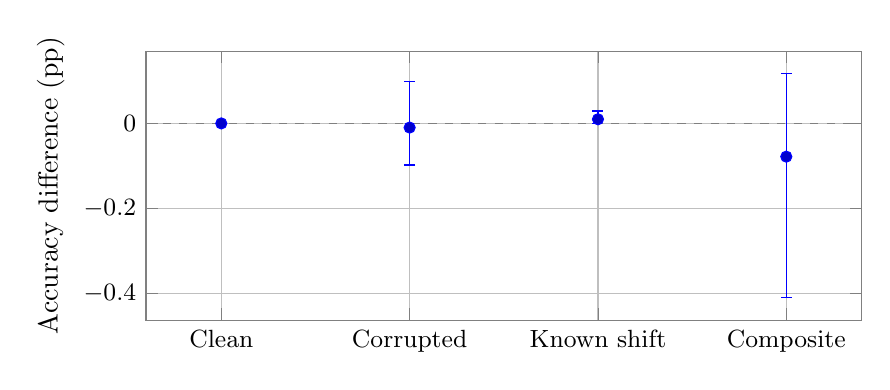
\begin{tikzpicture}\begin{axis}[width=.88\linewidth,height=5cm,
ylabel={Accuracy difference (pp)},xtick={0,1,2,3},
xticklabels={Clean,Corrupted,Known shift,Composite},xmin=-.4,xmax=3.4,
grid=major,axis line style={gray},tick label style={font=\small}]
\addplot+[only marks,mark=*,error bars/.cd,y dir=both,y explicit] coordinates {
(0,0.0) += (0,0.0) -= (0,0.0)
(1,-0.009765625) += (0,0.10742187500000001) -= (0,0.087890625)
(2,0.009765625) += (0,0.01953125) -= (0,0.009765625)
(3,-0.078125) += (0,0.1953125) -= (0,0.33203125000000006)};
\addplot[dashed,gray,domain=-.4:3.4] {0};
\end{axis}\end{tikzpicture}
\caption{Adaptive robust minus the development-selected control. Error bars
show descriptive 95\% paired dataset-cluster bootstrap intervals. Only the
composite contrast is the improvement primary; its practical threshold is +2 pp.}
\end{figure}

\begin{table}[ht]\centering\small
\caption{Protected accuracy (percent), averaged across ten cells. Selection aliases vary by development cell; all arms share bank predictions.}
\begin{tabular}{lrrrr}\toprule
Arm & Clean & Corrupted & Known shift & Composite \\\midrule
adaptive erm & 100.00 & 93.56 & 99.99 & 99.67 \\
adaptive robust & 100.00 & 93.54 & 99.99 & 99.62 \\
adaptive robust no penalty & 100.00 & 93.57 & 99.98 & 99.58 \\
constant erm & 100.00 & 93.19 & 99.99 & 99.76 \\
constant robust & 100.00 & 93.19 & 99.99 & 99.77 \\
direct erm & 100.00 & 93.52 & 99.99 & 99.53 \\
direct robust & 100.00 & 93.51 & 99.98 & 99.54 \\
expert 0 & 99.98 & 50.21 & 75.25 & 63.89 \\
expert 1 & 99.99 & 49.71 & 75.21 & 62.64 \\
expert 2 & 100.00 & 49.82 & 75.36 & 67.90 \\
expert 3 & 100.00 & 69.87 & 84.07 & 94.69 \\
expert 4 & 99.99 & 49.70 & 74.67 & 74.98 \\
fixed & 100.00 & 82.35 & 99.87 & 99.83 \\
reference & 100.00 & 92.94 & 99.99 & 99.75 \\
selected control & 100.00 & 93.55 & 99.98 & 99.70 \\
semantic & 100.00 & 92.94 & 99.99 & 99.75 \\
uniform & 100.00 & 78.28 & 99.50 & 99.38 \\
\bottomrule\end{tabular}\end{table}


\subsection{Ablations and competing explanations}
Reference selection chose semantic routing in all ten cells. Final control
selection chose direct ERM five times, direct robust four times, and constant
robust once. Improvement over the original reference can therefore arise from
additional fitting on new correction data. The primary candidate does not
establish an advantage over that competing explanation.

Adaptive ERM scores 99.6680\% on composite shift, modestly above adaptive robust
at 99.6191\%. Constant robust reaches 99.7656\%, and fixed routing reaches
99.8340\%. These are descriptive secondary observations, not retrospectively
selected primary winners. Fixed routing scores only 82.3535\% on familiar
corruption versus 93.5449\% for adaptive robust, demonstrating regime dependence.
Uniform routing scores 78.2813\% on familiar corruption and 99.3848\% on composite
shift. Neither a global ranking nor the best protected arm replaces the
frozen primary.

Removing the adaptive robust penalty yields 99.5801\% composite accuracy,
slightly below the penalized arm. Adaptive robust also exceeds direct robust
there (99.5410\%), while constant robust remains higher. These differences do
not establish that example-dependent intervention or worst-group training is
necessary. No adjusted secondary significance claim is made.

\subsection{Probability quality and action quality differ}
On composite shift, adaptive robust reduces reference NLL from 0.11085 to
0.10705 and Brier score from 0.02675 to 0.02562 while lowering accuracy. Its ECE
is 0.09130 versus reference 0.09619. Selected control remains better on all
three: NLL 0.10352, Brier 0.02448, ECE 0.08927. Probability quality can improve
relative to a reference without producing more correct decisions or beating a
stronger control. NLL improvement is not proof of an accuracy gain.

On familiar corruption, candidate NLL is 0.22352 versus reference 0.24456 and
selected control 0.22013. Candidate Brier is 0.09981 versus 0.11134 and 0.09879;
candidate ECE is 0.07376 versus 0.07699 and 0.06776. These secondary metrics
reinforce the extra-training explanation rather than isolate adaptive superiority.

\subsection{Intervention failure analysis}
\begin{table}[ht]\centering\small
\caption{Adaptive-robust intervention against the frozen reference. Counts sum ten cells (two initializations share each dataset).}
\begin{tabular}{lrrrr}\toprule Regime & Mean $\alpha$ & Rescues & Harms & Changes \\\midrule
clean & 0.4410 & 0 & 0 & 0 \\
corrupted & 0.6969 & 130 & 68 & 215 \\
known shift & 0.6094 & 0 & 0 & 0 \\
composite shift & 0.6758 & 9 & 22 & 31 \\
\bottomrule\end{tabular}\end{table}

Mean mixture weight rises above its initial 0.1: approximately 0.441 on clean,
0.697 on familiar corruption, 0.609 on known shift, and 0.676 on composite
shift. This is a probability-mixture weight, not a decision-change rate. The
penalty does not keep mean mixture weight near its initial 0.1. Its coefficient is a soft
tradeoff against NLL, not a hard constraint or correctness detector.

On composite shift, nine rescues and 22 harms yield
$(9-22)/10240=-0.00126953$ accuracy relative to reference, exactly the recorded
$-0.126953$ percentage-point reference contrast. There are 31 changed decisions.
On familiar corruption, 130 rescues and 68 harms yield
$62/10240=0.00605469$, or $+0.605469$ points. Of 215 changed predictions, 17
change from one wrong answer to another. Counts include two initializations of
the same five datasets and are not 10,240 independent experimental units.
Clean and known-shift decisions are unchanged from reference despite substantial
probability mixing.

Adaptive correction helps some familiar-corruption reference errors but
introduces more errors than it repairs under reserved shift. The familiar gain is matched by simpler continued-training controls; no
additional adaptive advantage is established. The evidence does not causally identify
whether the penalty, representation, optimization, expert correlations, or
shift configuration causes the failure. Those explanations require successor tests.

\section{Benchmark ceiling and scientific interpretation}
The selected control achieves 99.6973\% on the protected primary regime.
Even perfect prediction could improve that observed accuracy by only 0.3027
percentage points, below the registered two-point threshold. This ceiling was
identified after protected inspection. We retain the threshold and negative
result. Lowering the requirement or selecting a harder protected subset now
would invalidate confirmation.

The study does not support the promised practical gain, and its point estimate
is unfavorable. It also cannot establish the absence of a useful adaptive
mechanism on harder, separately defined data. The test is valid as the registered
comparison but has poor discriminatory scope for a two-point improvement in
this near-saturated regime. A future benchmark should establish task difficulty
and corrective opportunity on development evidence before freezing an untouched
confirmation set.

\section{Preserved predecessor chronology}
\begin{table}[ht]\centering\small
\caption{Preserved routing contrasts in percentage points. Endpoints differ;
this is a chronology, not a common learning curve. All listed primaries failed.}
\begin{tabular}{llrr}\toprule
Study & Endpoint/comparator & Delta & 95\% interval \\\midrule
v2 & Corrupt selective / uniform & $-4.69$ & $[-9.53,0.16]$ \\
v3 & Corrupt selective / semantic & $-1.25$ & $[-2.81,0.31]$ \\
v4 & Corrupt accuracy / semantic & $-6.82$ & $[-7.71,-5.89]$ \\
v5 & Reserved shift / core semantic & $-0.068$ & $[-0.244,0.107]$ \\
EditCLEVR & Shifted / selected control & $-0.005$ & $[-0.015,0]$ \\
v6 & Composite / selected control & $-0.078$ & $[-0.410,0.117]$ \\\bottomrule
\end{tabular}\end{table}
Earlier ledgers and the consolidated manuscript remain unchanged. In v4,
expanded corruption coverage improved semantic corrupted accuracy by 27.42
points, and semantic routing exceeded learned fixed routing by 10.21 points.
Removing its counterfactual penalty changed the relevant comparison by only
about 0.01 points. These are bounded secondary observations.

The separate v5 temporal primary remains supported within its synthetic task:
clean residual MSE was 0.014566 versus 0.071332 for the preceding predictor,
a 79.58\% reduction. Residual-minus-persistence was $-0.015398$ with interval
$[-0.015830,-0.014920]$. This is temporal-prediction evidence, not routing
improvement. V5 and EditCLEVR raw remote archives remain pending local retrieval.
Their recorded aggregate/provenance findings are preserved, not independently
reconstructed in this study.

\section{Discussion and next falsifiable direction}
The positive engineering outcome is a functioning, source-bound experiment with
strong controls and retained negative evidence. The narrower scientific
observation is that a useful familiar-regime reference correction need not be
a better shifted-regime policy. Direct mixture-NLL training combined with this
conservative correction did not establish the desired advantage. This study
does not isolate the earlier correctness-score-to-mixture proxy mismatch as
the cause.

A defensible successor would first measure, using development data alone,
which experts rescue each other's errors and whether a gate has information
to predict those rescues. It would use a task whose baseline leaves room for
the declared practical effect, compare to continued-training and constant
controls again, and test a materially different mechanism for distinguishing
rescue from harm. Harder inputs alone are not an improvement. Each change needs
a predicted consequence and an untouched confirmation set. No such successor
is executed or promoted here.

\section{Limitations, ethics, and reproducibility}
The five independent units are generator seeds, not independent natural-world
datasets. Signals are synthetic and redundant; three text experts share an
input channel. Perturbation types are historically known. Capacity differs
between arms, intervals use only five clusters, and no model-size scaling,
broad sensitivity sweep, real-world benchmark, or independent retraining is
included. Saturation especially limits the practical-improvement test. These
limits preclude general capability, safety, production, or state-of-the-art
claims. Zero of six Olympus families is promoted.

Scientific source, predictions, checkpoints, JSON reports, protocols, and the
verified archive accompany the artifact. The execution environment is recovered
by checking out \texttt{18a7052} and its lockfile. Later publication commits
patch Vite, certifi, and Pillow after release audits; they do not change frozen
model, generator, protocol, or tests. Results are not silently attributed to
the patched environment. The standalone renderer regenerates tables and
PGFPlots source from retained JSON without Torch.

The repository is publicly viewable under its existing proprietary license;
public availability does not grant unrestricted reuse. External reproduction
or redistribution must respect that license or obtain the copyright holder's
permission. No personal data or human-subject experiments are introduced.
The supplied style is retained byte-for-byte and the predecessor's author
display name is preserved. This manuscript is not submitted to arXiv or peer
reviewed. Independent source and arithmetic review is distinct from independent
experimental reproduction.

\section{Conclusion}
Conservative adaptive routing did not improve the frozen composite-shift
primary over a strong development-selected control. Nonregression passed and
familiar-corruption reference accuracy improved, but continued-training
controls matched that gain. The registered study closes with a negative
result, retained evidence, and a narrower successor question about corrective
opportunity and rescue-versus-harm prediction.

\appendix
\section{Artifact map and reproduction commands}
The study directory is \texttt{research/olympus\_routing\_v6}.
\texttt{protocol.json} is the authoritative contract;
\texttt{campaign-evidence.zip} retains all raw tensors and checkpoints;
\texttt{EVIDENCE\_RECEIPT.json} records the externally verified archive digest.
The unpacked \texttt{retained-campaign/routing-v6-campaign} contains the
contract, scientific freeze, summary, verification receipt, and development
and protected reports. Restore raw tensors from the ZIP after a Git clone.

\noindent\begin{minipage}{\linewidth}
For an authorized reproduction in the frozen checkout, use the locked environment
and new output directories:

\begin{verbatim}
uv sync --locked --all-extras
.venv/bin/python -m scripts.run_conservative_routing_v6 qualify \
  --output artifacts/qualification-NEW
.venv/bin/python -m scripts.run_conservative_routing_v6 run \
  --output artifacts/campaign-NEW \
  --qualification artifacts/qualification-NEW
.venv/bin/python -m scripts.run_conservative_routing_v6 verify \
  --output artifacts/campaign-NEW
\end{verbatim}
\end{minipage}

The public commands enforce resource and hard wall-time limits. Directly calling
the internal worker is not an admitted reproduction procedure. An additional
scientific execution must be separately recorded, not a search for a favorable
replacement result.

\section{Review and correction trail}
Pre-execution independent review found and repaired inherited frozen gradients
in copied alternatives, incomplete bank checkpoint replay, acceptance of
self-consistently rewritten predictions, and an unbound environment contract.
Artificial tamper tests cover the repairs. Protocol versions 6.0.0 and 6.0.1
remain retained; 6.0.2 was frozen before scientific data generation. Prospective
methods and their hashes are retained at the execution commit. Later wording
corrections clarify copied weights, separate backbone parameters, protected-only
replay, and inference-cost scope without changing the tested mechanism. The
flaw audit records outstanding scientific limits alongside engineering repairs.
